% \documentclass{article}

% \usepackage[utf8]{inputenc}
% \usepackage{amsmath}
% \usepackage{graphicx}
% \usepackage{booktabs}
% \usepackage{array}
% \usepackage{geometry}\geometry{a4paper, margin=1in}
% \usepackage{hyperref}
% \usepackage{parskip}

% \title{Architectural Description: Human Benchmark \\ \Large Information View}
% \author{Generated by AI Software Architect Assistant}
% \date{\today}

% \begin{document}

% \maketitle

% \tableofcontents

\section{Introduction to the Information View}

This Information View describes the way that the Human Benchmark system stores, manipulates and manages data.

\section{Core Architectural Elements of the Information View}

\subsection{Information Structure and Content}

The Human Benchmark system's information structure centers around several key data entities that are fundamental to its operation. Rather than detailing every attribute, this view focuses on the architecturally significant entities and their relationships.

\subsubsection{Key Data Entities}

Note this diagram only shows the new data entities that will be created to implement the new feature and those that are closley related, but whose purpose is not clear(The User entity is not shown, etc.). The diagram uses Crowfoot notation for ER diagrams.
Only a diagram for the static model is shown, as such the information flow model and information lifecycle model will be described by text as they are extremly trivial. Other models such as volumetric, metadata, information quality and information ownership will not be covered as they are not relevant to chats or it is obvious as for what kind of model is used due to the nature of the change being implemented(The owner of a message is its sender, etc.).

\begin{itemize}
    \item \textbf{Emojis}: Stores all emojis and messages that have these emojis.
    \item \textbf{Files}: Stores all of the files and a link to the message to which the file is attached.
    \item \textbf{GameRoomMessages}: This entity shows the messages that were sent to game rooms.
    \item \textbf{PrivateMessages}: This entity contains all messages that were sent in private chats.
    \item \textbf{Groups}: This entity stores all of the chat-groups that were created by users.
    \item \textbf{GroupMessages}: All of the messages sent to chat-groups.
    \item \textbf{GlobalMessages}: All of the messages that were sent in the global scope.
    \item \textbf{GameSessions}: All of the currently running game sessions(Used by game-room messages to store in which game-room the message was sent).
\end{itemize}

% TODO: DIAGRAM - Entity-Relationship diagram showing the key data entities and their relationships
% SUGGESTED_TYPE: Entity-Relationship Diagram (ERD)
% KEY_ELEMENTS_TO_DEPICT: User, Game, Target, Score, GameSession, GameUser entities with their relationships and key attributes
% STAKEHOLDER_FOCUS: Developers and maintainers who need to understand the data model
\begin{figure}[h!]
\centering
 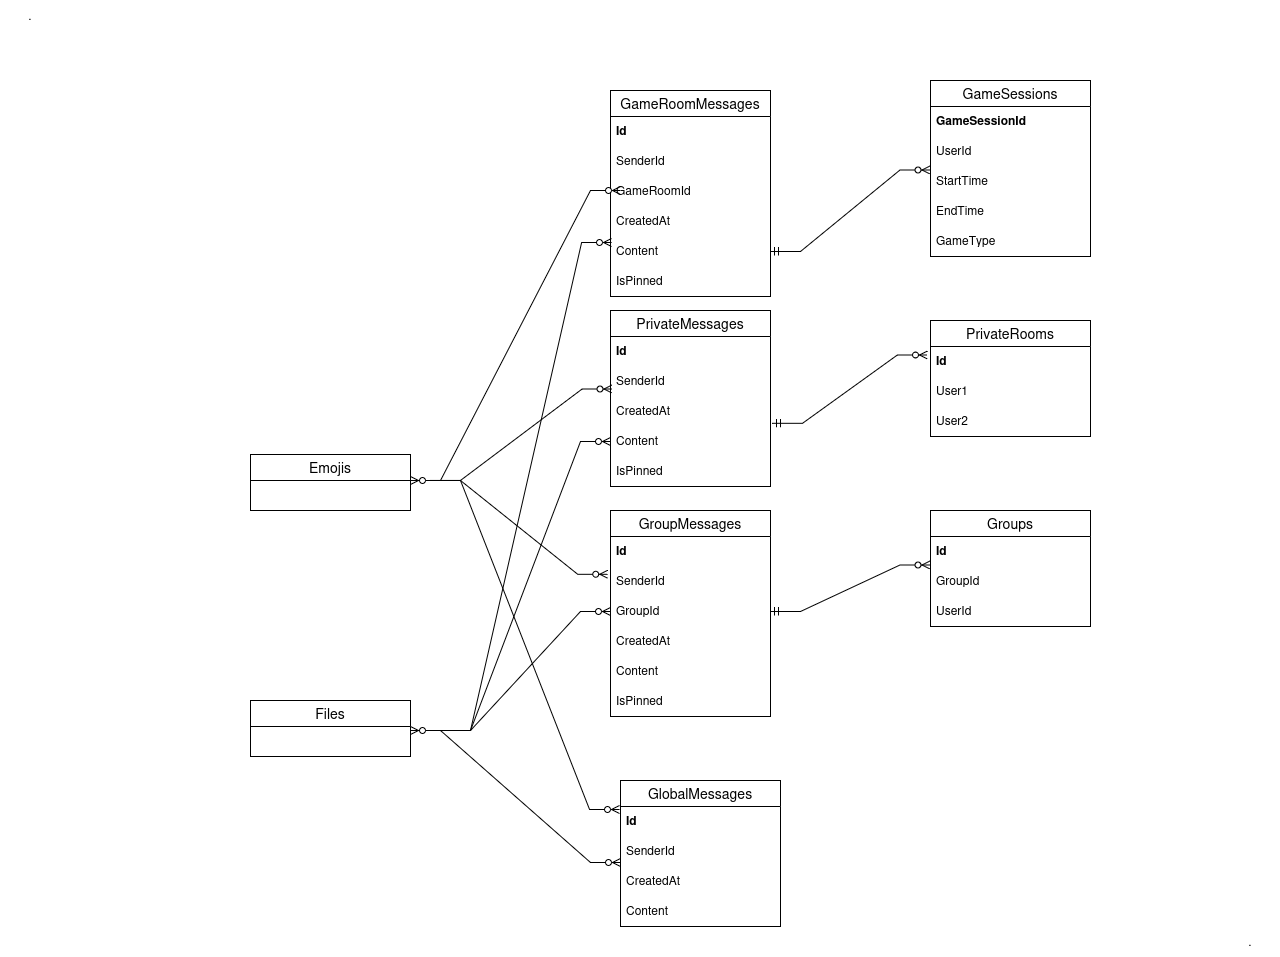
\includegraphics[width=0.9\textwidth]{4Lab2.drawio.png}
\caption{Entity-Relationship Diagram: Human Benchmark Core Data Model (Conceptual Placeholder)}
\label{fig:information_view_erd_overview}
\textit{Comment: This diagram should illustrate the main data entities and their relationships within the Human Benchmark system.}
\end{figure}

\subsection{Information Storage Model}
The data will be stored in a relational database. This is because they are widely used and have a way to unsure their quality such as the various normal forms and SQL.

\subsection{Information Flow}


\subsubsection{Real-time Communication Flows}

Since there are no system messages that use the chatting system, the data flow is as follows: the user sends a message which is sent to the real-time communication system which according to what kind of message it is it is forwarded to be sent to all users connected to the apropriate chat room and it is forwarded to the database for storage.

\subsection{Information lifecycles}

The messages can have the following states. There are two states that a message may have. Firstly a message may be pinned. This state is reversable, as in once a message has been pinned and its state has changed to pinned it can also be unpinned and the state of the message will revert. The second state that a message can have is the deleted state. Since our system does not delete messages by default the only way messages are deleted is following a users request to delete them.


\section{Perspective Priorities for the Information View}

\begin{table}[H]
\centering
\caption{Perspective Priorities for the Information View of Human Benchmark}
\label{tab:perspective_priorities_information}
\begin{tabular}{p{0.3\textwidth}p{0.15\textwidth}p{0.45\textwidth}}
% \toprule
\textbf{Architectural Perspective} & \textbf{Priority} & \textbf{Explanation} \\
% % \toprule
Accessibility & Low & The information object connected to the real-time messaging functionality is not related to accessibility from an architectural perspective. \\

Availability and Resilience & High &  Since we are implementing chatting in real time it is important that upon a users request old messages are loaded and new ones created effectively. \\

Development Resource & Medium & The database and information management implementation requires consideration of development effort. \\

Evolution & Low & The messages that will be created have little to no need to change over time. \\

Internationalization & Low & The Internationalization of chats is depend on users and users alone. There is no architectural way or need to Internationalize messages. \\



Security & Low & User messages have little to no need to have security measures in place for users. \\

Usability & Low & While usability is important for the system overall, it has limited direct impact on the underlying information model. \\
% % \toprule
\end{tabular}
\end{table}



% \end{document}
